

%%%%** Section 7.4
\subsection{Challenge Problem!  Amusement Park Ride}
A ride consists of a large arm with a rail mounted perpendicular to it.    The arm rotates about the $Z$ axis of a frame (1) with angular velocity $\omega$.  The stationary rest frame (sidewalk) is at frame (0).   At a given moment in time the arm forms the angle $\theta$ with $X_1$.     A chair and body restraint system slides along the rail back and forth with a sinusoidal motion between the two ends of the rail.

The victims/customers are thus subjected to velocities from both the rotating and sliding axes.

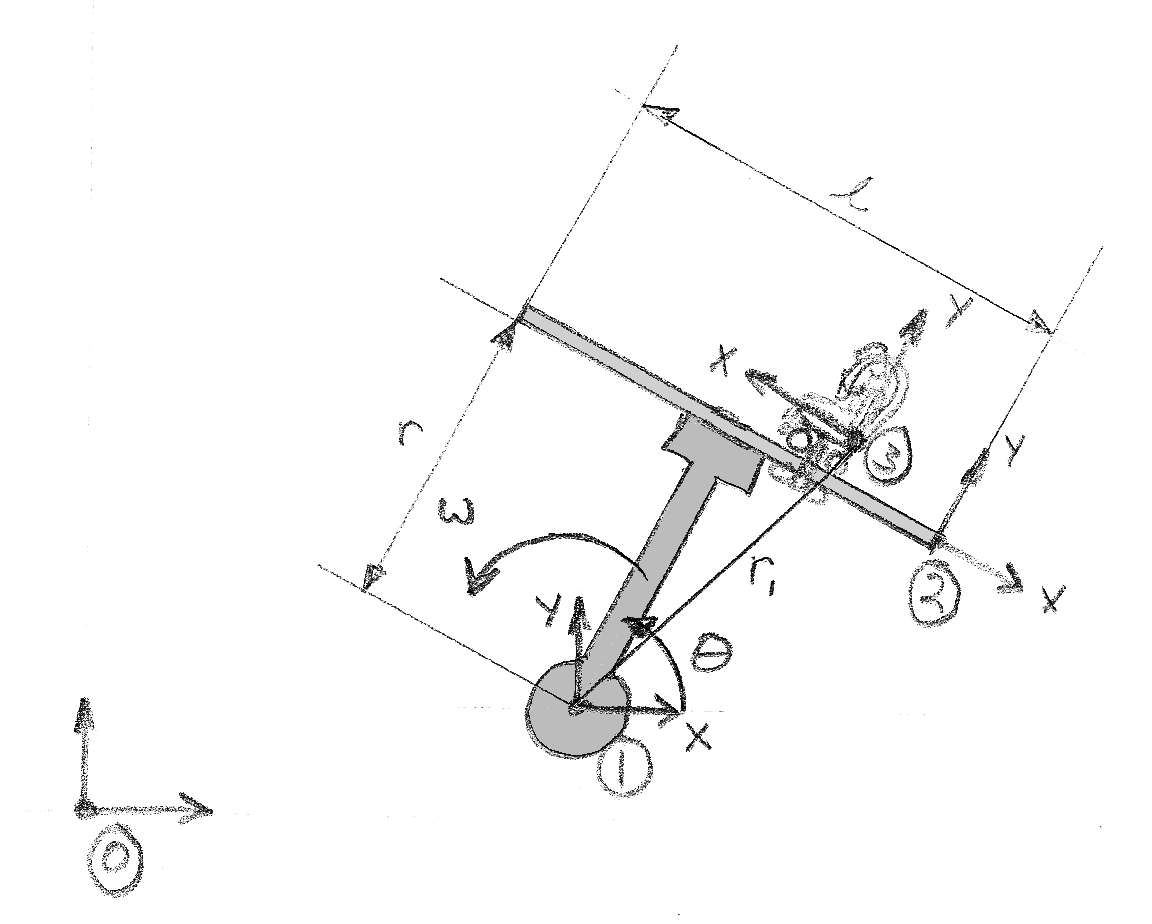
\includegraphics[width=4.0in]{00911.png}


The following facts are known (in addition to the above information):

\begin{itemize}

\item  $^A\left(^BV_C\right )$ means  the velocity of the origin of frame $C$, computed in frame $B$, and expressed in frame $A$.

\item Assume that ${^i_jR}$ or ${^i_jR}(t)$ is known for every $i,j$, and all the $Z_i$ are parallel at all times.

\item Assume the seat moves along the rail according to
\[
^2\left(^2P_3(t)\right) = \left [  -1*\left (l/2 + \frac{l}{2}\sin(2\pi t/3)\right), \: 0 , \: 0 \right]'
\]
and that the origin of (3) is directly on the track.

\item We will denote the velocity of the origin of frame $i$ by $V_i$.

\item A line connecting the origin of (1) with the origin of (3) has length $r_1$.


\end{itemize}


%%%%** Section 7.4.1
\subsubsection{} \label{blah}

Assume that $\omega=0,\; r=l/2$.  Find  $^0\left(^0V_3\right)$

<*n>
\begin{solution}

The only motion is due to the sled on the rail.
\[
^0\left(^0V_3\right) =  {^0_1R}\;{^1_2R}\; \frac{d}{dt} \left[ {^3X_2}(t)\right] =  {^0_1R}\;{^1_2R}\; (-\pi l/3)\cos(2\pi t/3)
\]
\end{solution}
<*>







%%%%** Section 7.4.2
\subsubsection{}  \label{blahblah}

 Find $^2\left(^0V_2\right)$

<*n>
\begin{solution}
\[
^2\left(^0V_2\right) = ^1\bmat0\\0\\ \omega \emat \times {^1r_1}
\]

\[
^2\left(^0V_2\right) = {^2_1R}\;\left[ \bmat 0\\0\\ \omega \emat \times {^1_2}R\bmat+l/2 \\+r\\0 \emat \right]
\]
\end{solution}
<*>




%%%%** Section 7.4.3
\subsubsection{}  Find $^2\left(^2V_3\right)$

<*n>
\begin{solution}
\[
^2\left(^2V_3\right) = {^2_3R}\; ^3\left(^2V_3\right)= \frac{d}{dt} \left[ {^2X_2}(t)\right] =  {^0_1R}\;{^1_2R}\;
\bmat (-\pi l/3)\cos(2\pi t/3)\\0\\0\emat
\]
\end{solution}
<*>



%%%%** Section 7.4.4
\subsubsection{}  Find $^0\left(^3V_3\right)$
<*n>
\begin{solution}
\[
^0\left(^3V_3\right) = \bmat 0&0&0\emat'
\]
\end{solution}
because the origin of frame 3 cannot move in frame 3. (There's one of these in every problem it seems!)

<*>

%%    Old problems no longer used in ICPS

%%%%** Section 7.4.5
\subsubsection{}  Find $^0\left(^0V_3\right)$

<*n>
\begin{solution}

There are two components of $V_3$ when computed in frame $0$:    1) the motion due to sliding along the rail. 2) The motion due to rotation by $\omega$.
\[
\left(^0V_3\right) = \left(^2V_3\right) + \bmat 0\\0\\\omega\emat\times r_1
\]
These are most easily available in frame 2 (see \ref{blahblah} and \ref{blah}.), but note that the angular velocity vector is the same in all frames because it points in the $Z$ direction.   Refering to the illustration below, the distance (A) in frame (3) is
\[
(A) = \frac{l}{2}\sin(\frac{2\pi}{3}t)
\]

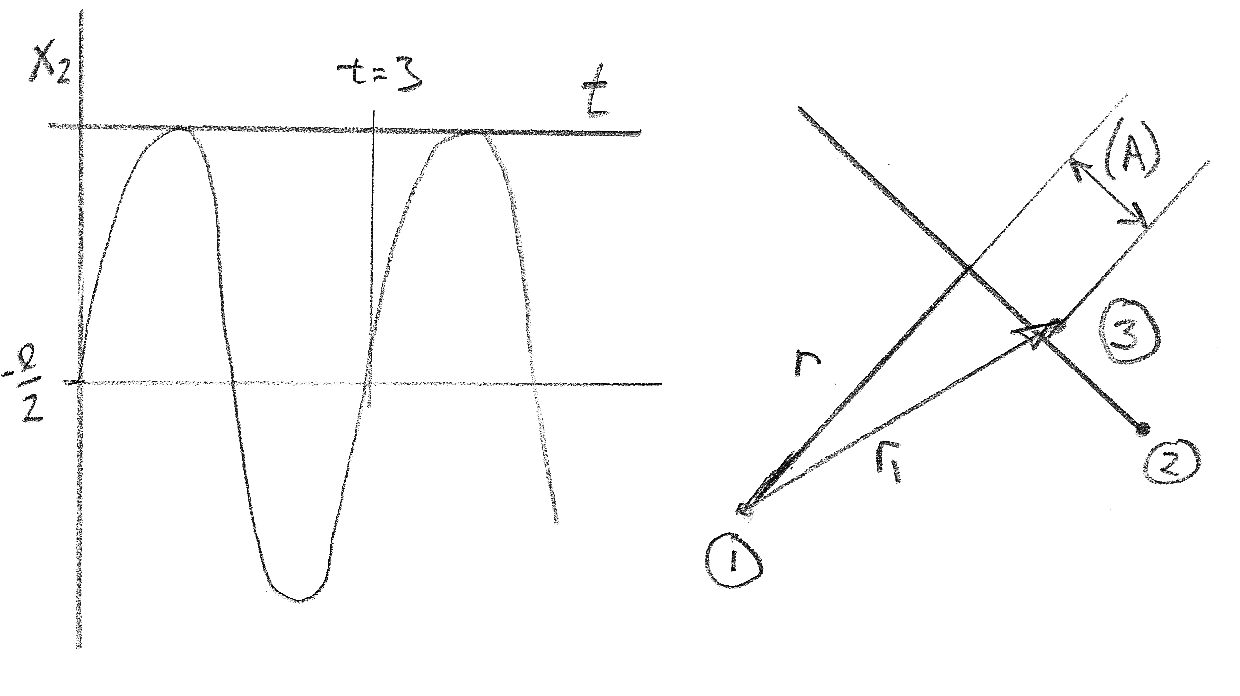
\includegraphics[width=5.0in]{00912.png}

the vector labeled $r_1$ can be then found in (3) and converted to (2)  by

\[
^3r_1 = {^2_3R}\;\bmat -l/2 \sin(\frac{2\pi}{3}t) \\-r \\ 0 \emat
\]
Therefore
\[
^3\left(^0V_3\right) = {^0_3R}\; ^2\left(^2V_3\right) +  \bmat 0\\0\\\omega\emat\times {^0_3R}\bmat -l/2 \sin(\frac{2\pi}{3}t) \\-r\\0 \emat
\]
\vspace{0.25in}
\[
^3\left(^0V_3\right) = {^0_3R}\; \left [ \bmat (-\pi l/3)\cos(2\pi t/3)\\0\\0\emat +  \bmat r\omega \\ -l/2 \sin(\frac{2\pi}{3}t)\omega \\0 \emat\right]
\]
\[
^3\left(^0V_3\right) = {^0_3R}\; \bmat (-\pi l/3)\cos(\frac{2\pi}{3}t)+ r\omega \\ -l/2 \sin(\frac{2\pi}{3}t)\omega \\0 \emat
\]

\end{solution}


